\documentclass[12pt,a4paper]{article}
\usepackage[utf8]{inputenc}
\usepackage[T2A]{fontenc}
\usepackage[russian]{babel}
\usepackage{graphicx}
\usepackage{booktabs}
\usepackage{longtable}
\usepackage{geometry}
\usepackage{float}
\usepackage{paracol}
\usepackage{src/title}
\usepackage[hidelinks]{hyperref}
\usepackage{listings}
\usepackage{xcolor}

\geometry{top=2cm, left=2cm, right=2cm, bottom=2cm}
\emergencystretch=1.5em
\sloppy

\title{Лабораторная работа №6. Логистическая регрессия}
\author{Ануфриев А.С. 465029}
\supervisor{Болдырева Елена Александровна}
\date{08.11.2026}

\abstract{
В работе выполнена реализация логистической регрессии ``с нуля'' на языке Python с использованием NumPy и Pandas для датасета пассажиров Титаника. Проведена предобработка данных, получена описательная статистика, исследовано влияние гиперпараметров (скорость обучения, количество итераций, метод оптимизации), оценены метрики классификации accuracy, precision, recall, F1-Score на тестовой выборке. Сделаны выводы о наилучших значениях гиперпараметров.
}
\keywords{логистическая регрессия, бинарная классификация, градиентный спуск, датасет Титаника, метрики классификации}

\begin{document}
\maketitle

\section{Цели и задачи}
Целью работы является реализация модели логистической регрессии для бинарной классификации без использования сторонних библиотек машинного обучения, исследование влияния гиперпараметров на качество модели и оценка её работы на тестовых данных.

Основные задачи:
\begin{enumerate}
\item загрузка и предобработка датасета пассажиров Титаника;
\item получение и визуализация описательной статистики по датасету (количество, среднее значение, стандартное отклонение, минимум, максимум, квантили);
\item разделение данных на обучающую и тестовую выборки;
\item реализация логистической регрессии ``с нуля'' (сигмоида, функция потерь log-loss, градиентный спуск, настраиваемая скорость обучения и количество итераций);
\item исследование влияния гиперпараметров: скорости обучения, количества итераций, метода оптимизации (градиентный спуск и оптимизация Ньютона);
\item оценка модели по метрикам accuracy, precision, recall, F1-Score на тестовой выборке для каждой комбинации гиперпараметров и выводы о наилучших значениях.
\end{enumerate}

\section{Исходные данные и предобработка}
В качестве исходных данных используется датасет пассажиров Титаника. Целевой признак --- \emph{Survived} (фактор выживания: 0 --- не выжил, 1 --- выжил). Числовые признаки: \emph{Pclass} (класс билета), \emph{Age} (возраст), \emph{SibSp} (число братьев/сестер и супругов на борту), \emph{Parch} (число родителей и детей на борту), \emph{Fare} (стоимость билета). Категориальные признаки: \emph{Sex} (пол), \emph{Embarked} (порт посадки). Признаки \emph{Name}, \emph{Ticket}, \emph{Cabin}, \emph{PassengerId} исключены из модели, поскольку не несут числовой информации для классификации.

Предобработка выполнялась в следующем порядке (чтобы избежать утечки информации из тестовой выборки в обучающую):
\begin{enumerate}
\item данные разделены на обучающую и тестовую выборки в соотношении 80/20 (фиксировано зерно генератора случайных чисел);
\item статистики для заполнения пропусков и стандартизации вычислены \emph{только} на обучающей выборке: медиана \emph{Age}, медиана \emph{Fare}, мода \emph{Embarked}, среднее и стандартное отклонение числовых признаков;
\item эти же статистики применены к тестовой выборке;
\item пропуски в \emph{Age} и \emph{Fare} заполнены медианой обучающей выборки, пропуски в \emph{Embarked} --- модой обучающей выборки;
\item признак \emph{Sex} закодирован (male --- 0, female --- 1), признак \emph{Embarked} закодирован one-hot кодированием (три отдельных признака для портов S, C, Q), что избегает искусственного порядка категорий;
\item числовые признаки стандартизированы (вычитание среднего, деление на стандартное отклонение обучающей выборки).
\end{enumerate}

После предобработки в модели используется 9 признаков (5 числовых + пол + 3 порта посадки one-hot). Датасет содержит 891 запись. Отсутствующие значения: в \emph{Age} --- 177, в \emph{Embarked} --- 2, в \emph{Cabin} --- 687 (признак исключён).

\section{Описательная статистика}
Для числовых признаков и целевой переменной получены показатели: количество, среднее, стандартное отклонение, минимум, 25-й, 50-й и 75-й квантили, максимум. Статистика приведена для explorative анализа на всех 891 записи после заполнения пропусков (параметры заполнения взяты из обучающей выборки). Для обучения модели статистики вычислялись только на обучающей выборке (как описано в разделе 2), чтобы избежать утечки данных.

\begin{table}[H]
\centering
\caption{Описательная статистика по датасету (все 891 запись).}
\label{tab:stats}
\begin{tabular}{lrrrrrrrr}
\toprule
Признак & Count & Mean & Std & Min & 25\% & 50\% & 75\% & Max \\
\midrule
Survived & 891 & 0.3838 & 0.4866 & 0.0 & 0.0 & 0.0 & 1.0 & 1.0 \\
Pclass & 891 & 2.3086 & 0.8361 & 1.0 & 2.0 & 3.0 & 3.0 & 3.0 \\
Age & 891 & 29.3616 & 13.0197 & 0.42 & 22.0 & 28.0 & 35.0 & 80.0 \\
SibSp & 891 & 0.5230 & 1.1027 & 0.0 & 0.0 & 0.0 & 1.0 & 8.0 \\
Parch & 891 & 0.3816 & 0.8061 & 0.0 & 0.0 & 0.0 & 0.0 & 6.0 \\
Fare & 891 & 32.2042 & 49.6934 & 0.0 & 7.91 & 14.45 & 31.0 & 512.33 \\
\bottomrule
\end{tabular}
\end{table}

Доля выживших пассажиров составляет около 38,4\%. Распределение целевой переменной представлено на рисунке~\ref{fig:survived}.

\begin{figure}[H]
\centering
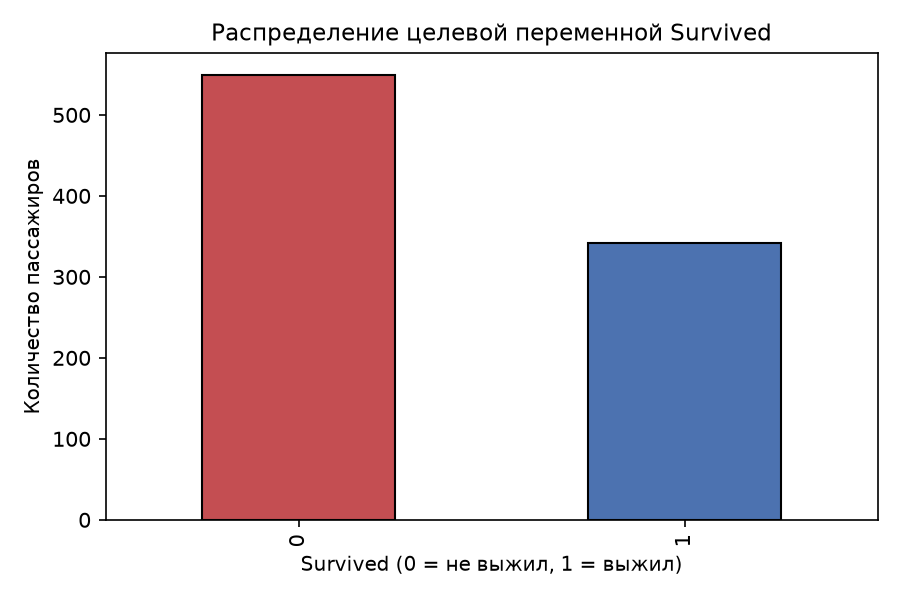
\includegraphics[width=0.6\textwidth]{../graphics/lab6_survived.png}
\caption{Распределение целевой переменной Survived.}
\label{fig:survived}
\end{figure}

Гистограммы числовых признаков приведены на рисунке~\ref{fig:histograms}.

\begin{figure}[H]
\centering
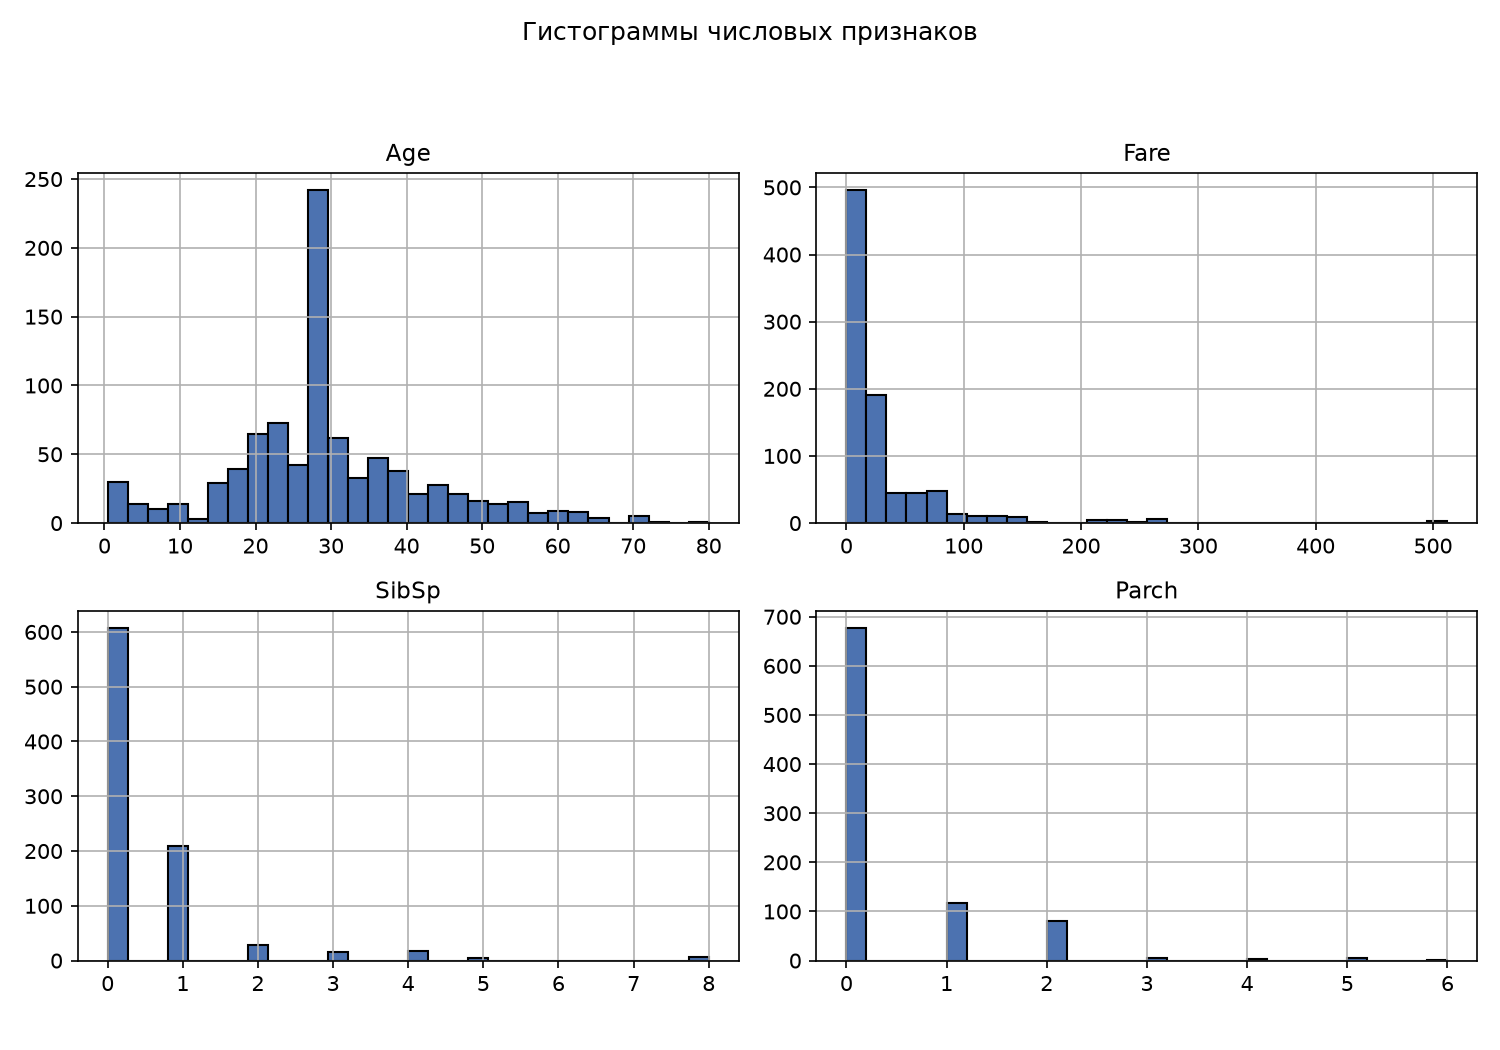
\includegraphics[width=0.9\textwidth]{../graphics/lab6_histograms.png}
\caption{Гистограммы числовых признаков датасета.}
\label{fig:histograms}
\end{figure}

\section{Метод логистической регрессии}
Логистическая регрессия моделирует вероятность принадлежности объекта к положительному классу с помощью сигмоидной функции:

\begin{equation}
\sigma(z) = \frac{1}{1 + e^{-z}}, \qquad p = \sigma(Xw),
\end{equation}

где \(X\) --- матрица признаков со столбцом смещения, \(w\) --- вектор весов, \(p\) --- предсказанная вероятность выживания.

Функция потерь (логарифмические потери, log-loss):

\begin{equation}
L(w) = -\frac{1}{N}\sum_{i=1}^{N}\left[y_i\ln p_i + (1-y_i)\ln(1-p_i)\right].
\end{equation}

Обучение выполняется градиентным спуском:

\begin{equation}
w \leftarrow w - \frac{\eta}{N}X^T(p-y),
\end{equation}

где \(\eta\) --- скорость обучения (learning rate). Для оптимизации Ньютона используется вторая производная:

\begin{equation}
w \leftarrow w - H^{-1}\nabla L(w),
\end{equation}

где \(H = \frac{1}{N}X^T W X\) --- гессиан функции потерь, \(W = \mathrm{diag}(p_i(1-p_i))\) [1, 2]. Гиперпараметры (скорость обучения, число итераций, метод оптимизации) варьируются вручную.

\section{Ход работы}
Данные разделены на обучающую и тестовую выборки в соотношении 80/20 (фиксировано зерно генератора случайных чисел для воспроизводимости): 712 записей на обучение, 179 записей на тестирование. Разбиение выполнено один раз, стратификация не применялась.

Проведено исследование гиперпараметров: три значения скорости обучения (0.01, 0.1, 0.5), три числа итераций (100, 500, 1000) и два метода оптимизации (градиентный спуск, оптимизация Ньютона). Для каждой комбинации модель обучается на обучающей выборке, а качество оценивается на тестовой.

\section{Результаты}
Результаты исследования гиперпараметров приведены в таблице~\ref{tab:hp}.

\begin{table}[H]
\centering
\caption{Качество модели на тестовой выборке для комбинаций гиперпараметров.}
\label{tab:hp}
\begin{tabular}{lrrrrrrr}
\toprule
Метод & lr & Iter. & Loss & Acc & Prec. & Rec. & F1 \\
\midrule
GD & 0.01 & 100 & 0.6340 & 0.6983 & 0.6341 & 0.4000 & 0.4906 \\
GD & 0.01 & 500 & 0.5490 & 0.7207 & 0.6744 & 0.4462 & 0.5370 \\
GD & 0.01 & 1000 & 0.5115 & 0.7430 & 0.6863 & 0.5385 & 0.6034 \\
GD & 0.1 & 100 & 0.5118 & 0.7430 & 0.6863 & 0.5385 & 0.6034 \\
GD & 0.1 & 500 & 0.4503 & 0.7765 & 0.6866 & 0.7077 & 0.6970 \\
GD & 0.1 & 1000 & 0.4449 & 0.7765 & 0.6866 & 0.7077 & 0.6970 \\
GD & 0.5 & 100 & 0.4503 & 0.7765 & 0.6866 & 0.7077 & 0.6970 \\
GD & 0.5 & 500 & 0.4442 & 0.7765 & 0.6866 & 0.7077 & 0.6970 \\
GD & 0.5 & 1000 & 0.4442 & 0.7765 & 0.6866 & 0.7077 & 0.6970 \\
Newton & -- & 100 & 0.4442 & 0.7765 & 0.6866 & 0.7077 & 0.6970 \\
Newton & -- & 500 & 0.4442 & 0.7765 & 0.6866 & 0.7077 & 0.6970 \\
Newton & -- & 1000 & 0.4442 & 0.7765 & 0.6866 & 0.7077 & 0.6970 \\
\bottomrule
\end{tabular}
\end{table}

Наилучший результат по F1-Score показывает градиентный спуск с learning rate 0.1 и 500 итерациями: accuracy 0.7765, precision 0.6866, recall 0.7077, F1-Score 0.6970 (TP = 46, TN = 93, FP = 21, FN = 19). Увеличение learning rate свыше 0.1 и увеличение числа итераций свыше 500 не приводят к улучшению метрик: loss стабилизируется, а значения accuracy, precision, recall и F1-Score остаются прежними. Метод оптимизации Ньютона сходится за немногие итерации, но не даёт преимущества в точности на тестовой выборке по сравнению с градиентным спуском.

Кривая обучения для лучшей комбинации приведена на рисунке~\ref{fig:curve}. Тепловая карта зависимости F1-Score от скорости обучения и числа итераций для градиентного спуска --- на рисунке~\ref{fig:heatmap}.

Матрица ошибок для лучшей комбинации (GD, lr = 0.1, 500 итераций) на тестовой выборке:

\begin{table}[H]
\centering
\caption{Матрица ошибок лучшей модели на тестовой выборке.}
\label{tab:confusion}
\begin{tabular}{lrr}
\toprule
 & Предсказано: не выжил & Предсказано: выжил \\
\midrule
На самом деле: не выжил & TN = 93 & FP = 21 \\
На самом деле: выжил & FN = 19 & TP = 46 \\
\bottomrule
\end{tabular}
\end{table}

\begin{figure}[H]
\centering
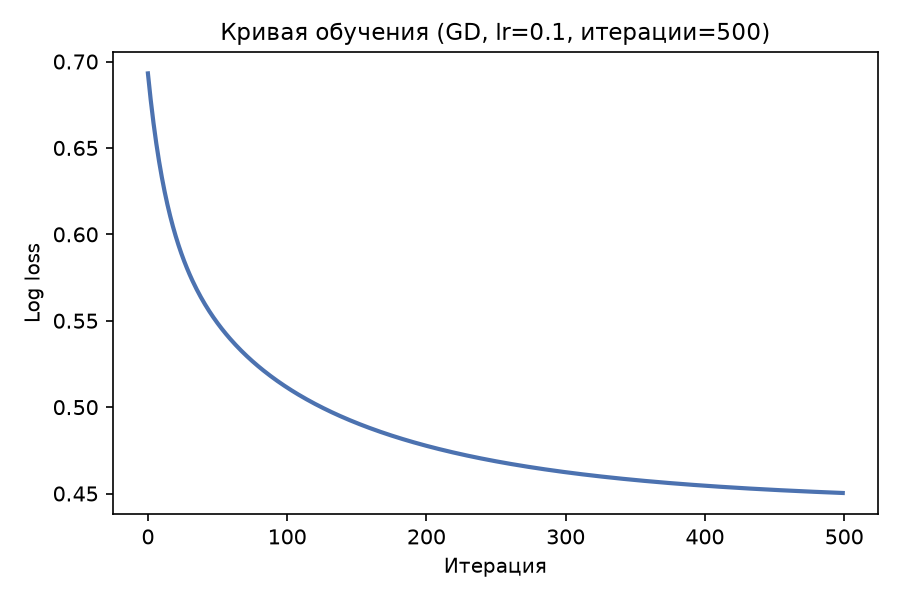
\includegraphics[width=0.6\textwidth]{../graphics/lab6_learning_curve.png}
\caption{Кривая обучения (градиентный спуск, lr = 0.1, 500 итераций).}
\label{fig:curve}
\end{figure}

\begin{figure}[H]
\centering
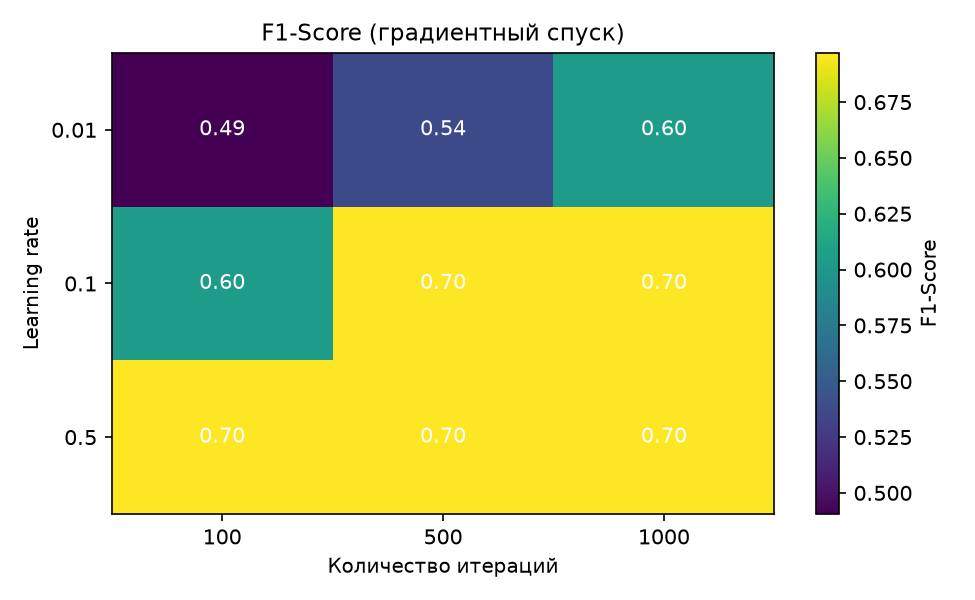
\includegraphics[width=0.7\textwidth]{../graphics/lab6_hyperparam_heatmap.png}
\caption{Зависимость F1-Score от learning rate и числа итераций (градиентный спуск).}
\label{fig:heatmap}
\end{figure}

\section{Ограничения}
\begin{itemize}
\item Качество модели оценено на одном случайном разбиении 80/20 без стратификации и без повторений; наилучшая комбинация гиперпараметров может зависеть от состава конкретной тестовой выборки.
\item Метрики получены для одного фиксированного разбиения (зерно генератора 42), поэтому абсолютные значения точности могут варьироваться при другом разбиении.
\end{itemize}

\section{Выводы}
\begin{enumerate}
\item Реализована логистическая регрессия ``с нуля'' на Python (NumPy/Pandas): сигмоида, log-loss, градиентный спуск с настраиваемой скоростью обучения и числом итераций, а также оптимизация Ньютона.
\item Проведена предобработка датасета Титаника без утечки данных: статистики для заполнения пропусков и стандартизации вычислены только на обучающей выборке и применены к тестовой.
\item Категориальный признак Embarked zakодирован one-hot кодированием, что избегает искусственного порядка категорий.
\item Данные разделены на обучающую (80\%) и тестовую (20\%) выборки.
\item Исследовано влияние гиперпараметров. Наилучшее качество по F1-Score (0.6970) достигается при learning rate 0.1, 500 итерациях и градиентном спуске.
\item Метод оптимизации Ньютона сходится быстро, но не даёт преимущества в точности на тестовой выборке по сравнению с градиентным спуском.
\item Увеличение learning rate свыше 0.1 и числа итераций свыше 500 не улучшает метрики: loss стабилизируется.
\item Классы несбалансированы: доля выживших 38,4\%, что снижает точность предсказания меньшего класса (выживших) при общем высоком accuracy.
\item Помимо данного отчёта, подготовлен отдельный документ с теоретическими сведениями по логистической регрессии и ответами на вероятные вопросы защиты.
\end{enumerate}

\section{Литература}
\begin{thebibliography}{9}
\bibitem{hosmer} Хосмер Д., Лемишоу С. Прикладная логистическая регрессия. --- М.: Вильямс, 2011.
\bibitem{bishop} Бишоп К. Распознавание образов и машинное обучение. --- М.: Бинар, 2010.
\bibitem{hastie} Хейстри Т., Тибширани Р., Фридман Дж. Элементы статистического обучения: освоение интеллектуального анализа данных. --- М.: Бином, 2010.
\bibitem{goodfellow} Гудфеллоу И., Бенгио Й., Курвилль А. Глубокое обучение. --- М.: Питер, 2018.
\end{thebibliography}

\section{Приложение}
В приложении приведены фрагменты реализации на Python, достаточные для воспроизведения метода (полный скрипт хранится отдельно от отчёта).

\begin{lstlisting}[language=Python, frame=single, basicstyle=\footnotesize\ttfamily]
import numpy as np
import pandas as pd

# Source data: Titanic passenger dataset (load from CSV)
data_file = 'data/train.csv'
df = pd.read_csv(data_file)

# Hyperparameters
lr = 0.1
n_iter = 500

# Split train/test BEFORE any preprocessing to avoid data leakage
np.random.seed(42)
idx = np.random.permutation(len(df))
n_train = int(0.8 * len(df))
train_idx = idx[:n_train]
test_idx = idx[n_train:]
df_train = df.iloc[train_idx].reset_index(drop=True)
df_test = df.iloc[test_idx].reset_index(drop=True)

# Statistics computed ONLY on train, then applied to test
age_median = df_train['Age'].median()
fare_median = df_train['Fare'].median()
embarked_mode = df_train['Embarked'].mode()[0]

df_train['Age'] = df_train['Age'].fillna(age_median)
df_train['Fare'] = df_train['Fare'].fillna(fare_median)
df_train['Embarked'] = df_train['Embarked'].fillna(embarked_mode)
df_test['Age'] = df_test['Age'].fillna(age_median)
df_test['Fare'] = df_test['Fare'].fillna(fare_median)
df_test['Embarked'] = df_test['Embarked'].fillna(embarked_mode)

# Encoding
df_train['Sex'] = (df_train['Sex'] == 'female').astype(int)
df_test['Sex'] = (df_test['Sex'] == 'female').astype(int)
emb_train = pd.get_dummies(df_train['Embarked'], prefix='Embarked')
df_train = pd.concat([df_train, emb_train], axis=1)
emb_test = pd.get_dummies(df_test['Embarked'], prefix='Embarked')
df_test = pd.concat([df_test, emb_test], axis=1)

features = ['Pclass', 'Sex', 'Age', 'SibSp', 'Parch', 'Fare',
            'Embarked_S', 'Embarked_C', 'Embarked_Q']

# Standardization using train statistics only
train_mean = df_train[features[:6]].mean()
train_std = df_train[features[:6]].std()
for c in features[:6]:
    df_train[c] = (df_train[c] - train_mean[c]) / train_std[c]
    df_test[c] = (df_test[c] - train_mean[c]) / train_std[c]

X_train = df_train[features].values.astype(float)
X_test = df_test[features].values.astype(float)
y_train = df_train['Survived'].values.astype(float)
y_test = df_test['Survived'].values.astype(float)

def sigmoid(z):
    return 1 / (1 + np.exp(-np.clip(z, -500, 500)))

def log_loss(y, p):
    eps = 1e-12
    p = np.clip(p, eps, 1 - eps)
    return -np.mean(y * np.log(p) + (1 - y) * np.log(1 - p))

def metrics(y_true, y_pred):
    tp = int(np.sum((y_pred == 1) & (y_true == 1)))
    tn = int(np.sum((y_pred == 0) & (y_true == 0)))
    fp = int(np.sum((y_pred == 1) & (y_true == 0)))
    fn = int(np.sum((y_pred == 0) & (y_true == 1)))
    acc = (tp + tn) / len(y_true)
    prec = tp / max(tp + fp, 1)
    rec = tp / max(tp + fn, 1)
    f1 = 2 * prec * rec / max(prec + rec, 1e-12)
    return acc, prec, rec, f1, tp, tn, fp, fn

# Gradient descent
Xb = np.c_[np.ones(len(X_train)), X_train]
w = np.zeros(Xb.shape[1])
for _ in range(n_iter):
    p = sigmoid(Xb @ w)
    grad = Xb.T @ (p - y_train) / len(y_train)
    w = w - lr * grad

# Newton optimization (second order, learning rate not required)
W = np.diag(p * (1 - p))
H = (Xb.T @ W @ Xb) / len(y_train)
w_newton = w - np.linalg.solve(H, grad)

# Predictions and metrics on test set
Xb_test = np.c_[np.ones(len(X_test)), X_test]
p_test = sigmoid(Xb_test @ w)
pred = (p_test >= 0.5).astype(int)
acc, prec, rec, f1, tp, tn, fp, fn = metrics(y_test, pred)
print(f'Accuracy={acc:.4f} Precision={prec:.4f}')
print(f'Recall={rec:.4f} F1={f1:.4f}')
print(f'TP={tp} TN={tn} FP={fp} FN={fn}')
\end{lstlisting}

\end{document}
